\begin{figure}[h!]
   \centering
   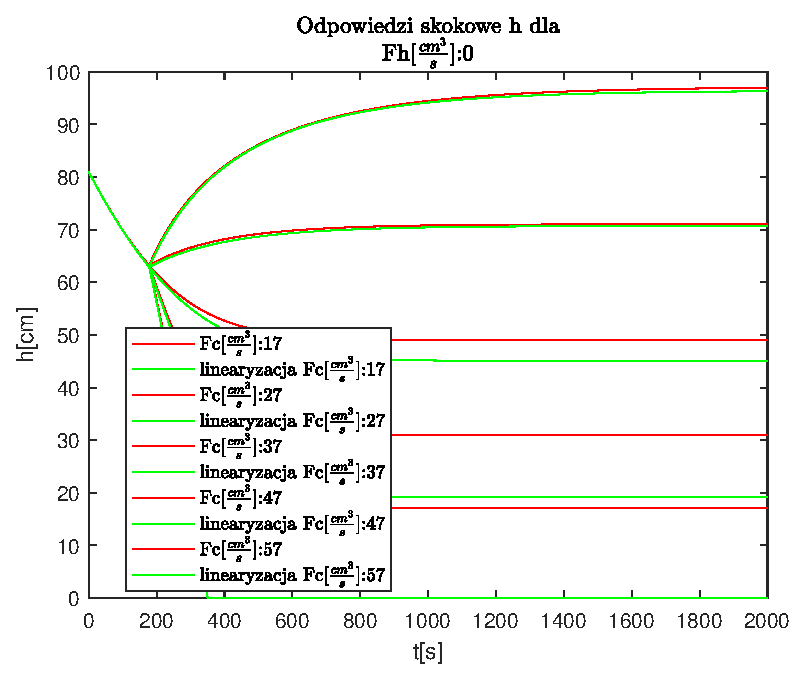
\includegraphics{img/step-responses/h/stepResponseHFh0.eps}
   \caption{Poziom cieczy w zbiorniku w odpowiedzi skokowej dla skoku Fh[$rac{cm^3}{s}$]: 0}
   \label{fig:stepResponseHFh0}
\end{figure}
            
\begin{figure}[h!]
   \centering
   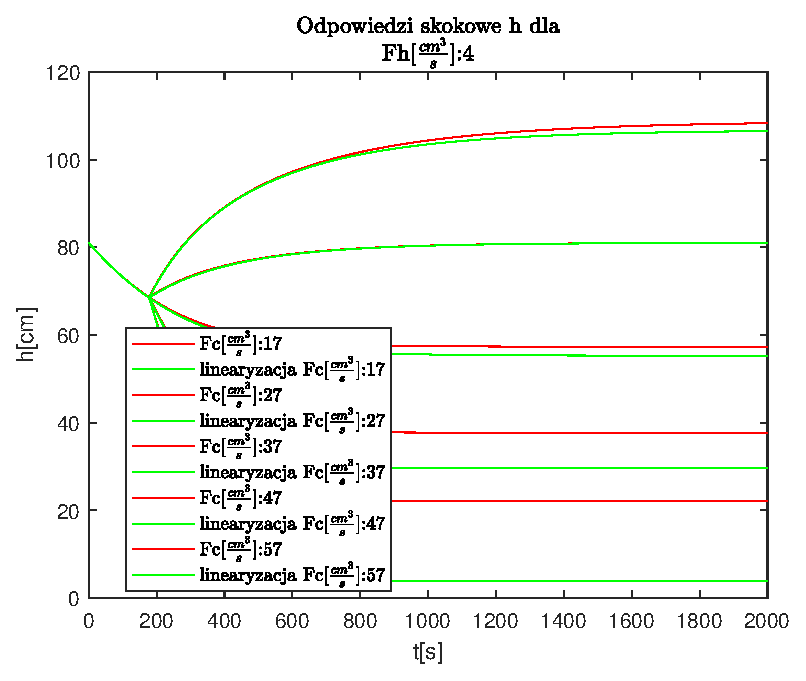
\includegraphics{img/step-responses/h/stepResponseHFh4.eps}
   \caption{Poziom cieczy w zbiorniku w odpowiedzi skokowej dla skoku Fh[$rac{cm^3}{s}$]: 4}
   \label{fig:stepResponseHFh4}
\end{figure}
            
\begin{figure}[h!]
   \centering
   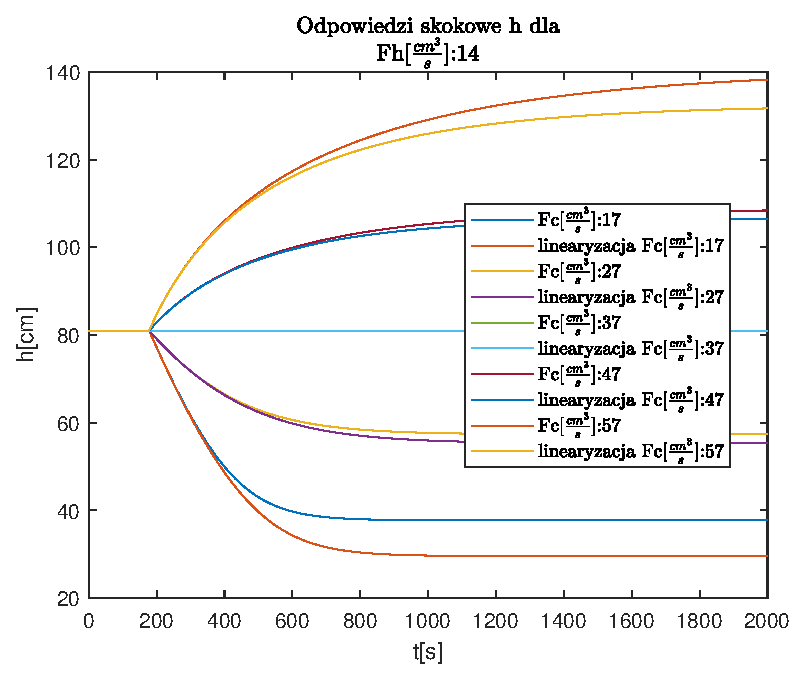
\includegraphics{img/step-responses/h/stepResponseHFh14.eps}
   \caption{Poziom cieczy w zbiorniku w odpowiedzi skokowej dla skoku Fh[$rac{cm^3}{s}$]: 14}
   \label{fig:stepResponseHFh14}
\end{figure}
            
\begin{figure}[h!]
   \centering
   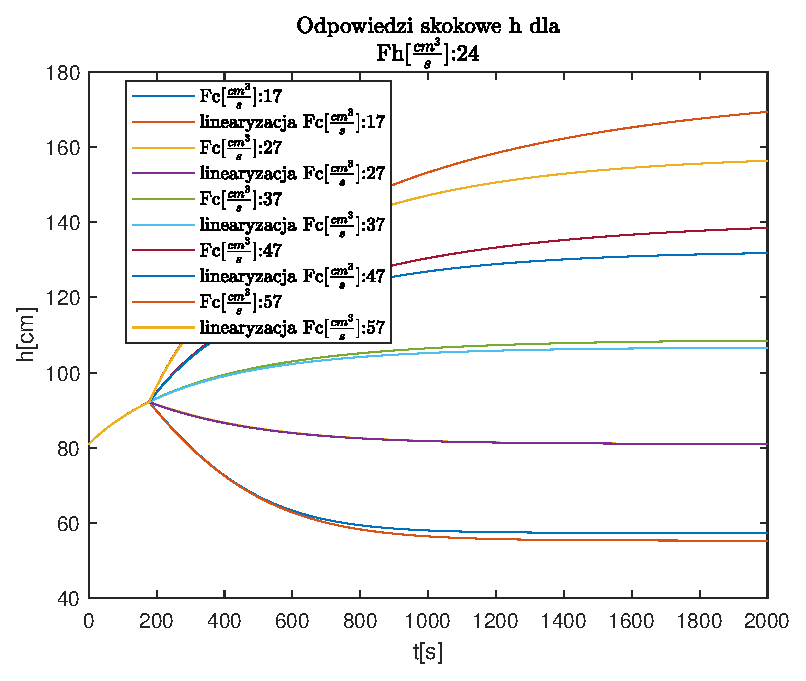
\includegraphics{img/step-responses/h/stepResponseHFh24.eps}
   \caption{Poziom cieczy w zbiorniku w odpowiedzi skokowej dla skoku Fh[$rac{cm^3}{s}$]: 24}
   \label{fig:stepResponseHFh24}
\end{figure}
            
\begin{figure}[h!]
   \centering
   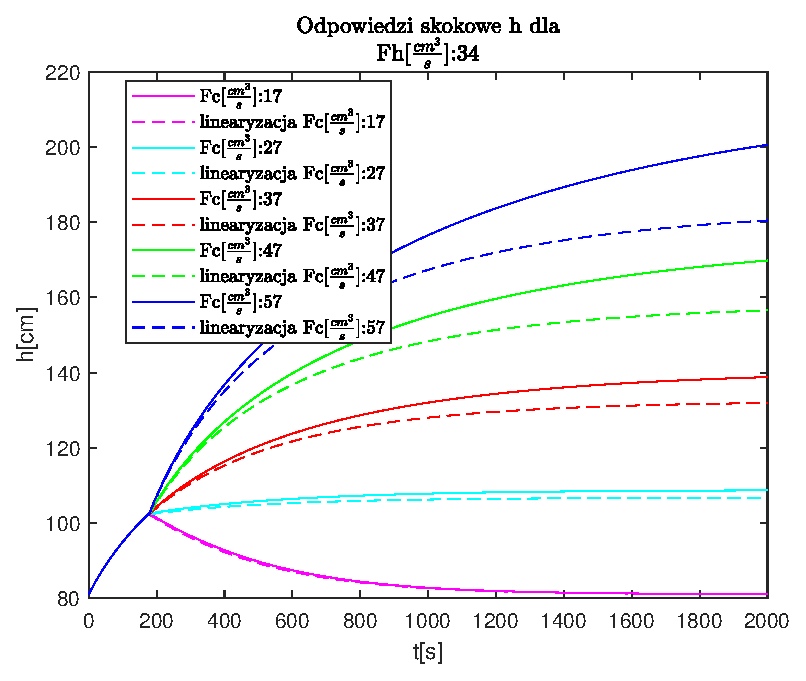
\includegraphics{img/step-responses/h/stepResponseHFh34.eps}
   \caption{Poziom cieczy w zbiorniku w odpowiedzi skokowej dla skoku Fh[$rac{cm^3}{s}$]: 34}
   \label{fig:stepResponseHFh34}
\end{figure}
            
